\begin{figure} % "[t!]" placement specifier just for this example
	\centering




	\begin{subfigure}{0.25\textwidth}
		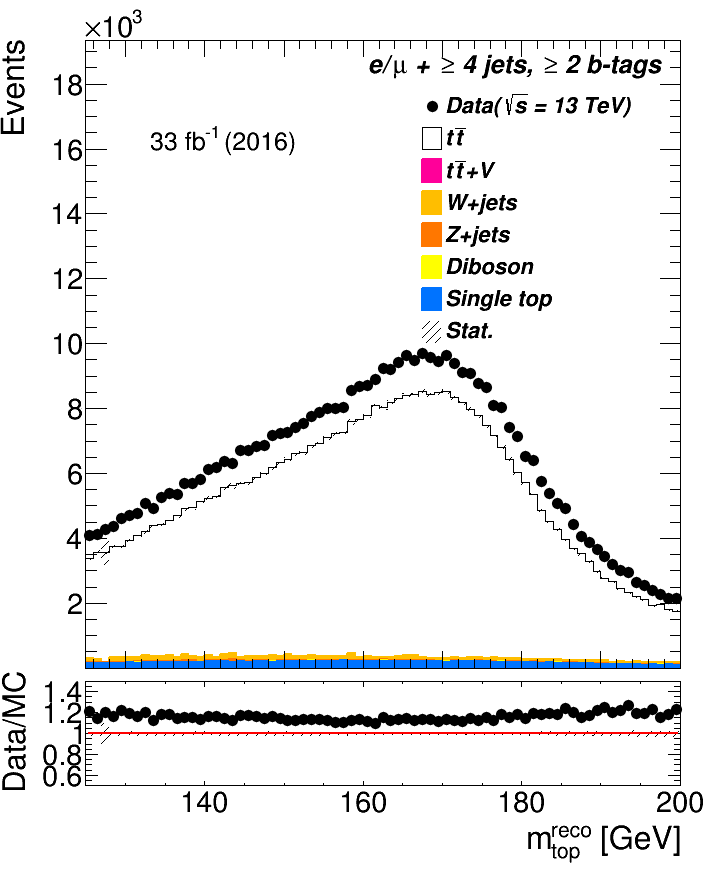
\includegraphics[width=\linewidth]{ControlPlots_emujets_2016_4incl_2incl//klf_window_mtop_reco_emujets_2016.png}
		\caption{Reconstructed hadronic top-quark mass $m_{\rm top}^{\rm reco}$.} \label{fig:K3}
	\end{subfigure}	\hspace*{0.5cm}
	\begin{subfigure}{0.25\textwidth}
		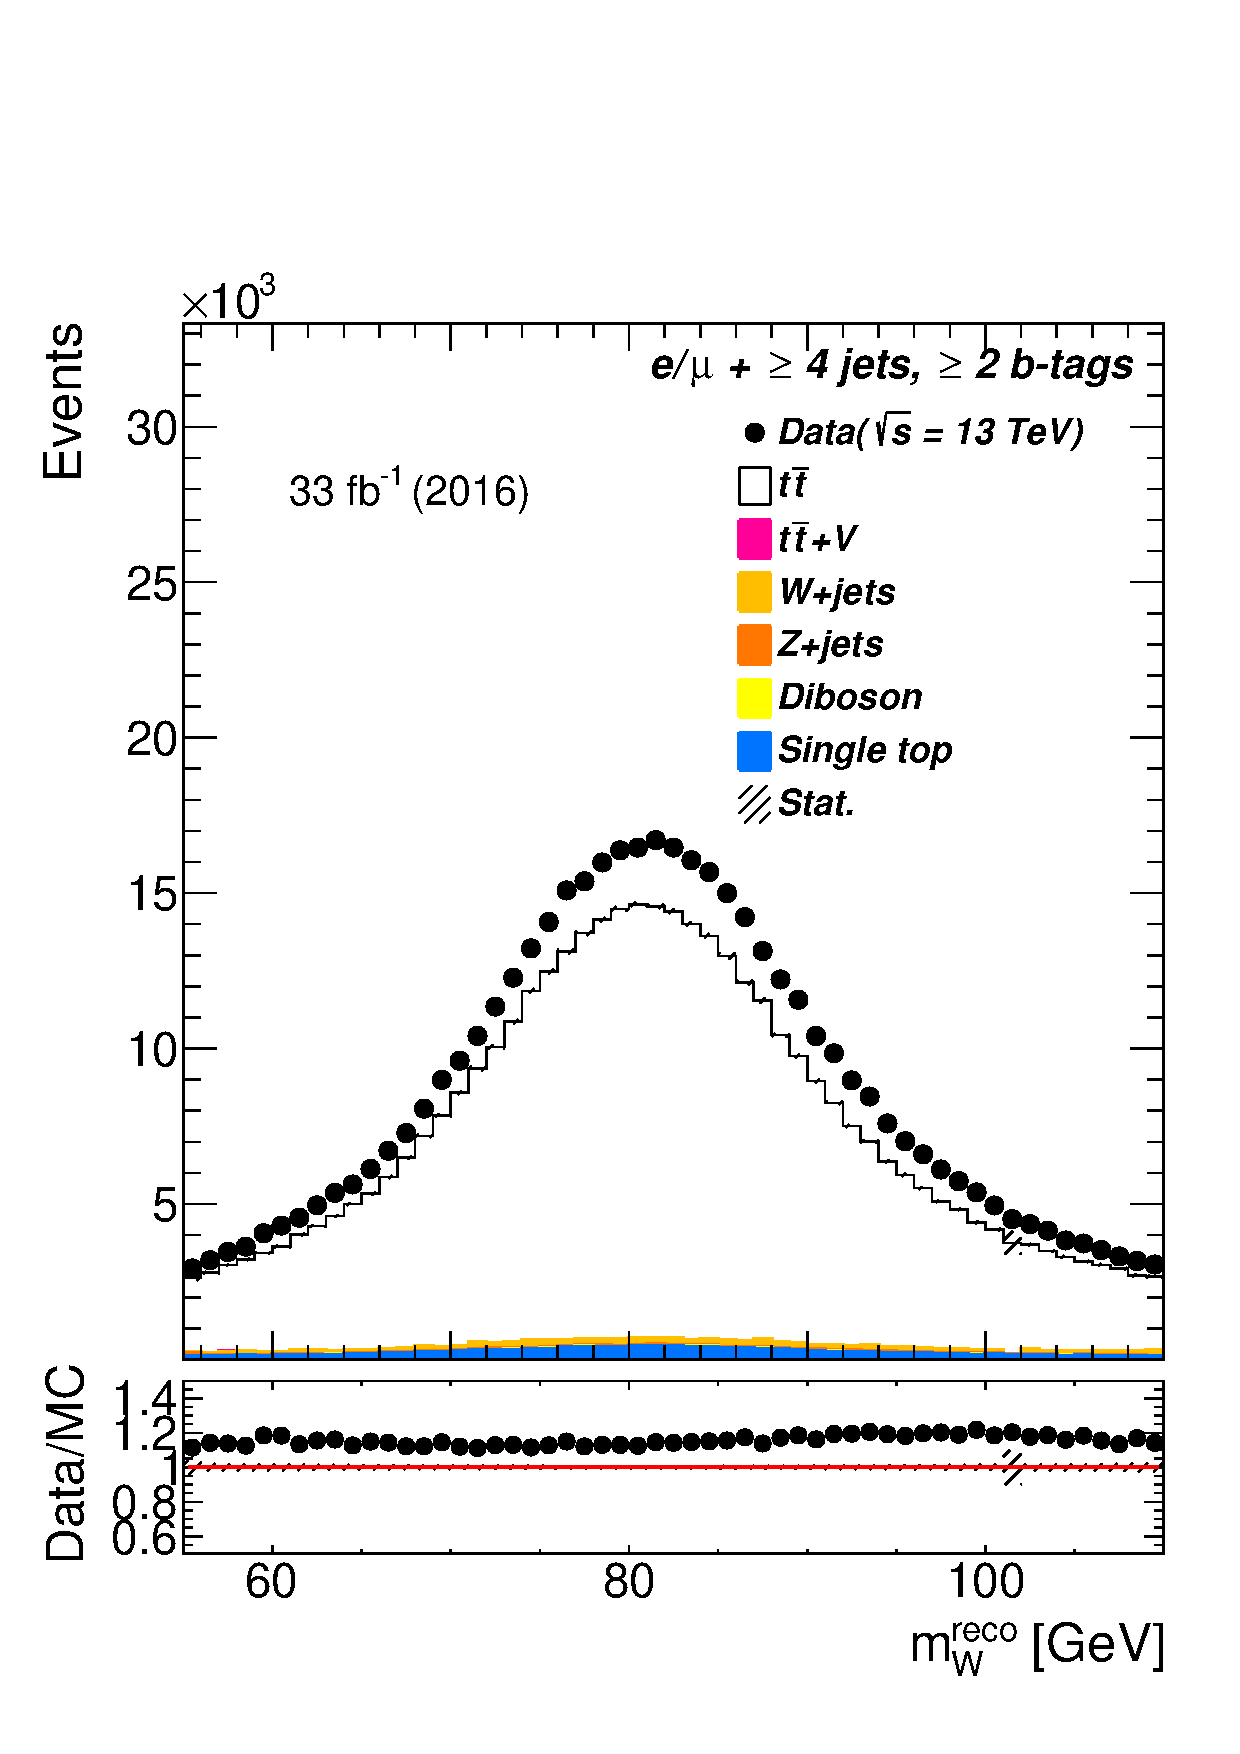
\includegraphics[width=\linewidth]{ControlPlots_emujets_2016_4incl_2incl/klf_window_mw_reco_emujets_2016.pdf}
		\caption{Reconstructed hadronic $W-boson$ mass $m_{\rm W}^{\rm reco}$.} \label{fig:K4}
	\end{subfigure}	\hspace*{0.5cm}	
	\begin{subfigure}{0.25\textwidth}
		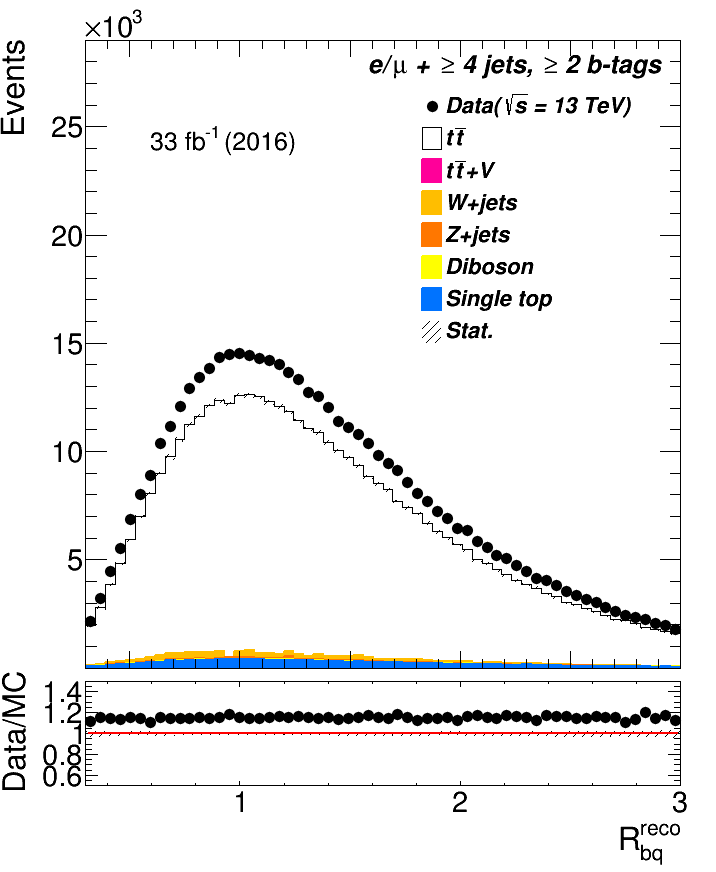
\includegraphics[width=\linewidth]{ControlPlots_emujets_2016_4incl_2incl/klf_window_rbq_reco_emujets_2016.png}
		\caption{Reconstructed $p_T$ ratio $R_{\rm bq}^{\rm reco}$.} \label{fig:K5}
	\end{subfigure}




\begin{subfigure}{0.25\textwidth}
	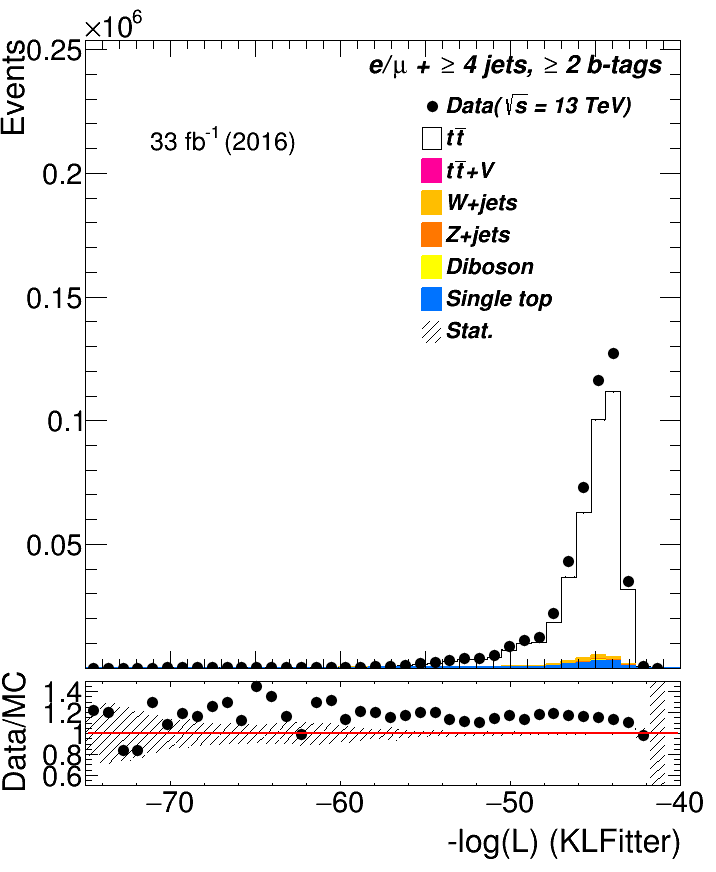
\includegraphics[width=\linewidth]{ControlPlots_emujets_2016_4incl_2incl/klf_LL_emujets_2016.png}
	\caption{The kinematic logarithmic \textsc{KLFitter} likelihood function.} \label{fig:K2}
\end{subfigure}\hspace*{0.5cm}	
	\begin{subfigure}{0.25\textwidth}
	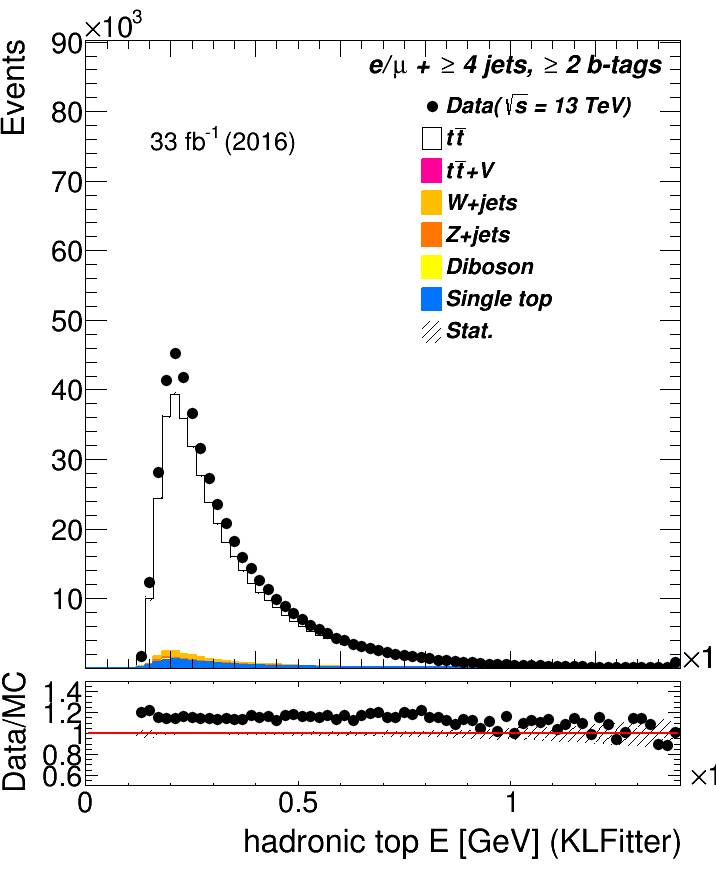
\includegraphics[width=\linewidth]{ControlPlots_emujets_2016_4incl_2incl/klf_topHad_E_emujets_2016.png}
	\caption{Energy of the hadronic top quark.} \label{fig:K7}
\end{subfigure}
\hspace*{0.5cm}
\begin{subfigure}{0.25\textwidth}
	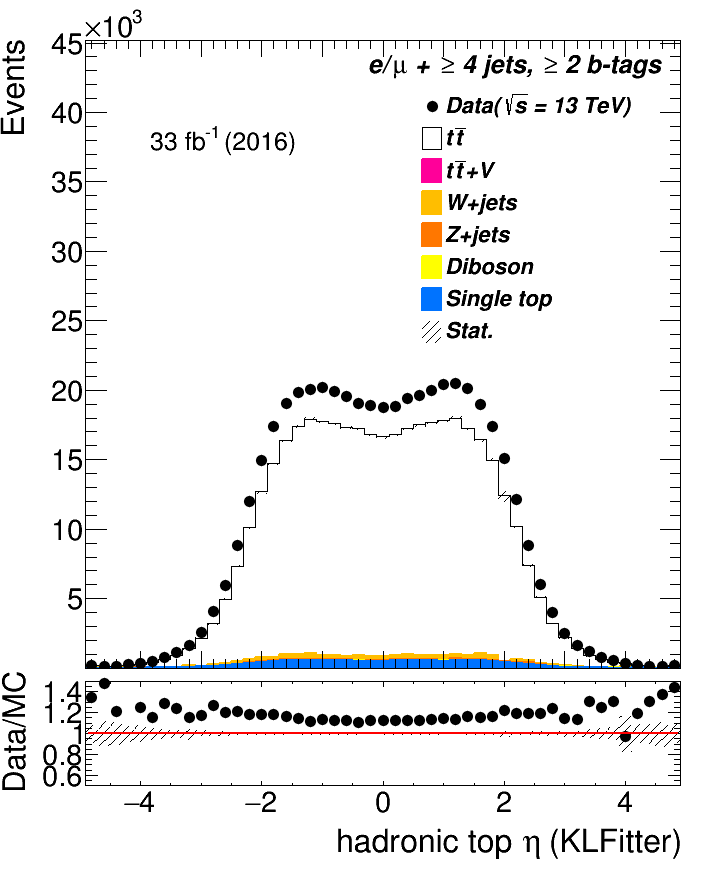
\includegraphics[width=\linewidth]{ControlPlots_emujets_2016_4incl_2incl/klf_topHad_eta_emujets_2016.png}
	\caption{$\eta$ of the hadronic top quark.} \label{fig:K8}
\end{subfigure}



	\begin{subfigure}{0.25\textwidth}
	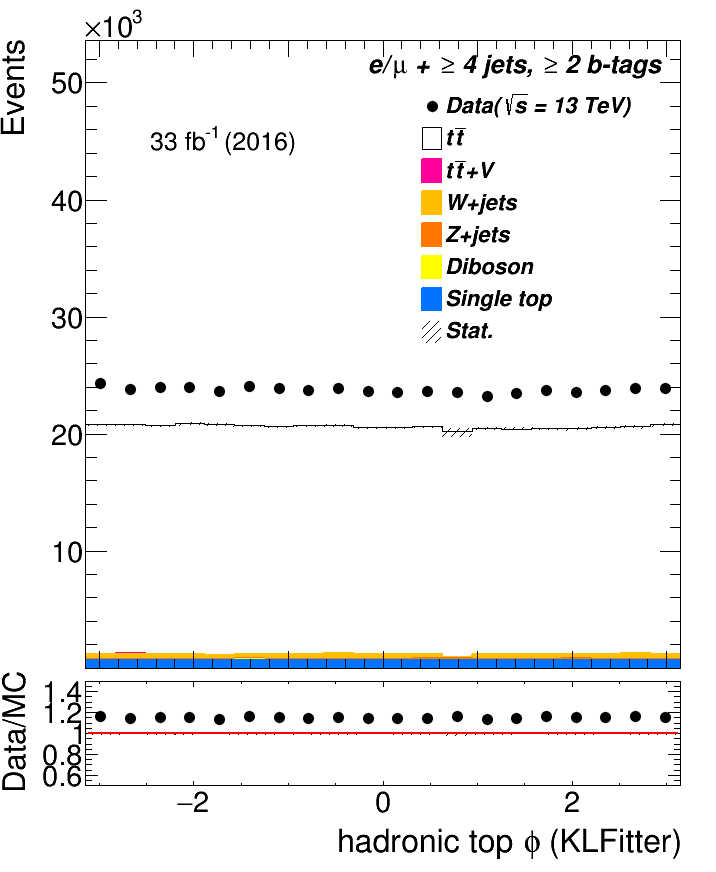
\includegraphics[width=\linewidth]{ControlPlots_emujets_2016_4incl_2incl/klf_topHad_phi_emujets_2016.png}
	\caption{$\phi$ of the hadronic top quark.} \label{fig:K9}
\end{subfigure}	
\hspace*{0.5cm}	
\begin{subfigure}{0.25\textwidth}
	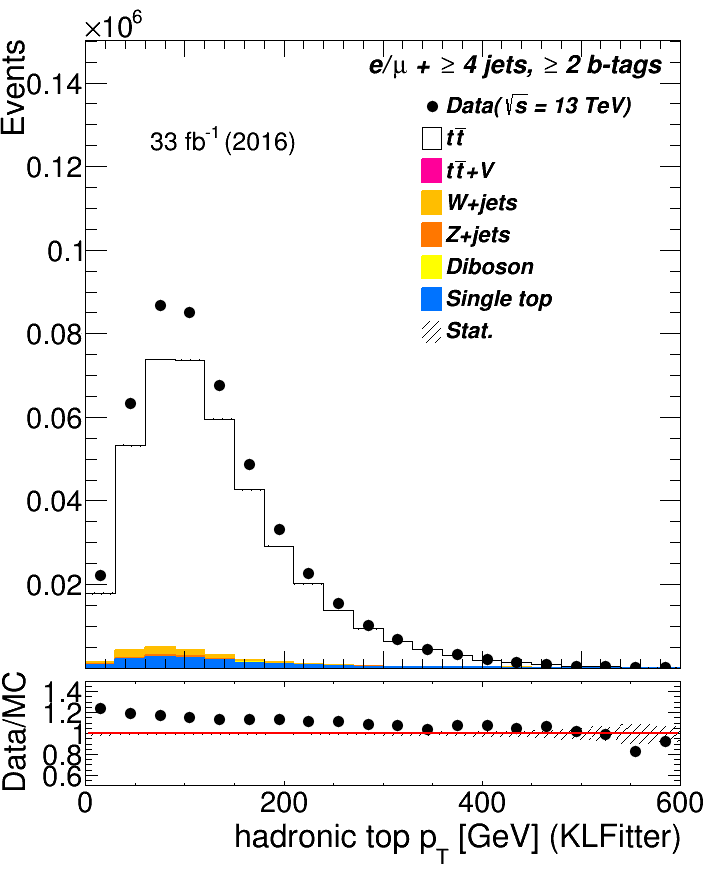
\includegraphics[width=\linewidth]{ControlPlots_emujets_2016_4incl_2incl/klf_topHad_pt_emujets_2016.png}
	\caption{Transverse momentum of the hadronic top quark.} \label{fig:K10}
\end{subfigure}\hspace*{0.5cm}
\begin{subfigure}{0.25\textwidth}
	\includegraphics[width=\linewidth]{ControlPlots_emujets_2016_4incl_2incl/klf_topLEP_E_emujets_2016.png}
	\caption{Energy of the leptonic top quark.} \label{fig:K11}
\end{subfigure}

\caption{Reconstructed global quantities, obtained with \textsc{KLFitter}. The black points represent the data, while the simulation is denoted by the solid histogram. The simulation of the different background processes are also shown by the coloured histograms. The data-simulation agreement is shown by the lower plot. Only statical errors are considered and the QCD-multijet background  is missing. The log-likelihood distribution is used by \textsc{KLFitter}, to obtain the best jet-patron assignment. The hadronic top-quark and  $W$-boson mass, as well as $R_{\rm bq}^{\rm reco}$ are very important quantities, which are generated from the event kinematics. If not mentioned different, the term hadronic or leptoinc, refer to the corresponding decay of the top-quark pair.}\label{klf100}
\end{figure}	



\begin{figure} % "[t!]" placement specifier just for this example
	\centering

	\begin{subfigure}{0.25\textwidth}
		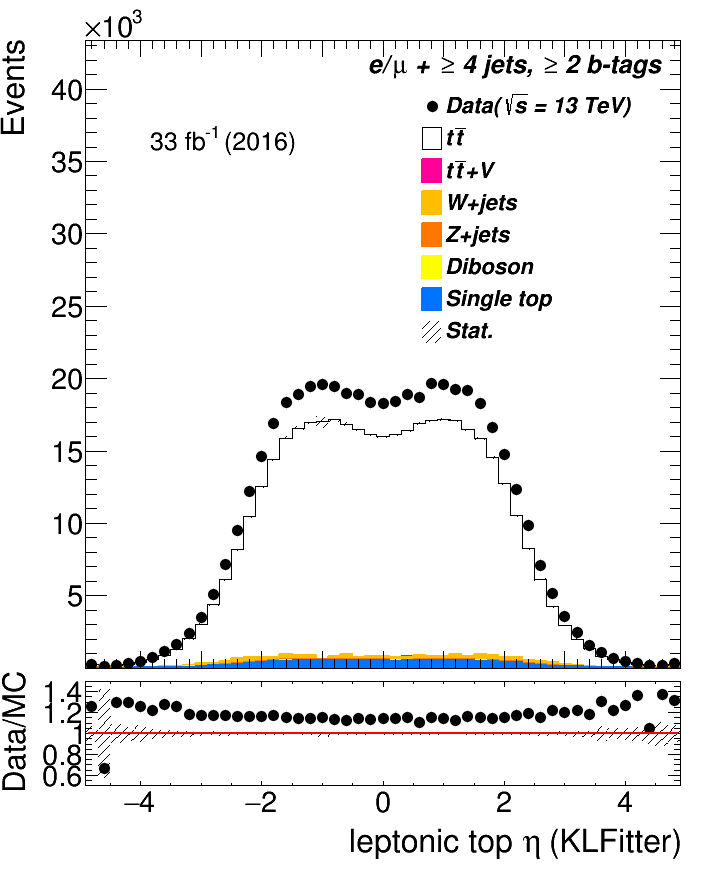
\includegraphics[width=\linewidth]{ControlPlots_emujets_2016_4incl_2incl/klf_topLep_eta_emujets_2016.png}
		\caption{$\eta$ of the leptonic top quark.} \label{fig:K12}
	\end{subfigure}	\hspace*{0.5cm}
	\begin{subfigure}{0.25\textwidth}
	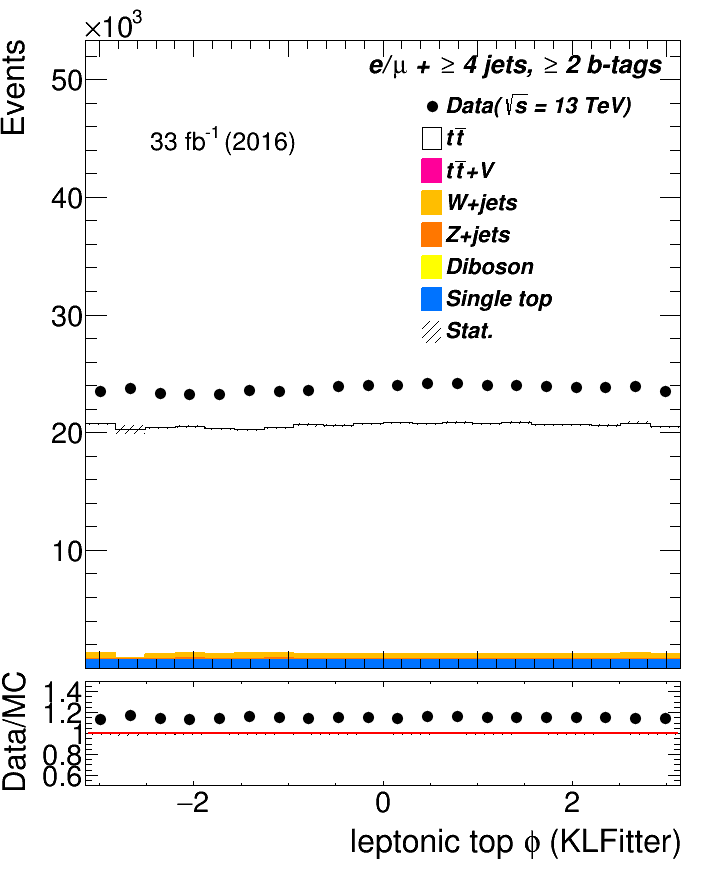
\includegraphics[width=\linewidth]{ControlPlots_emujets_2016_4incl_2incl/klf_topLep_phi_emujets_2016.png}
	\caption{$\phi$ of the leptonic top quark.} \label{fig:K13}
\end{subfigure}
\hspace*{0.5cm}
\begin{subfigure}{0.25\textwidth}
	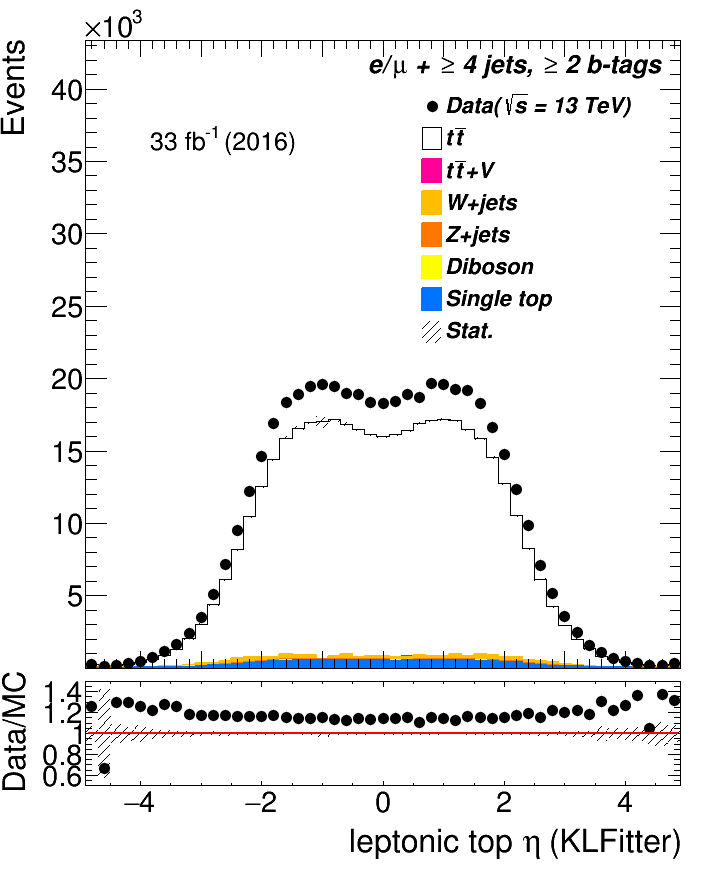
\includegraphics[width=\linewidth]{ControlPlots_emujets_2016_4incl_2incl/klf_topLep_eta_emujets_2016.png}
	\caption{$\eta$ of the leptonic top-quark.} \label{fig:K14}
\end{subfigure}



	
	
	\begin{subfigure}{0.25\textwidth}
		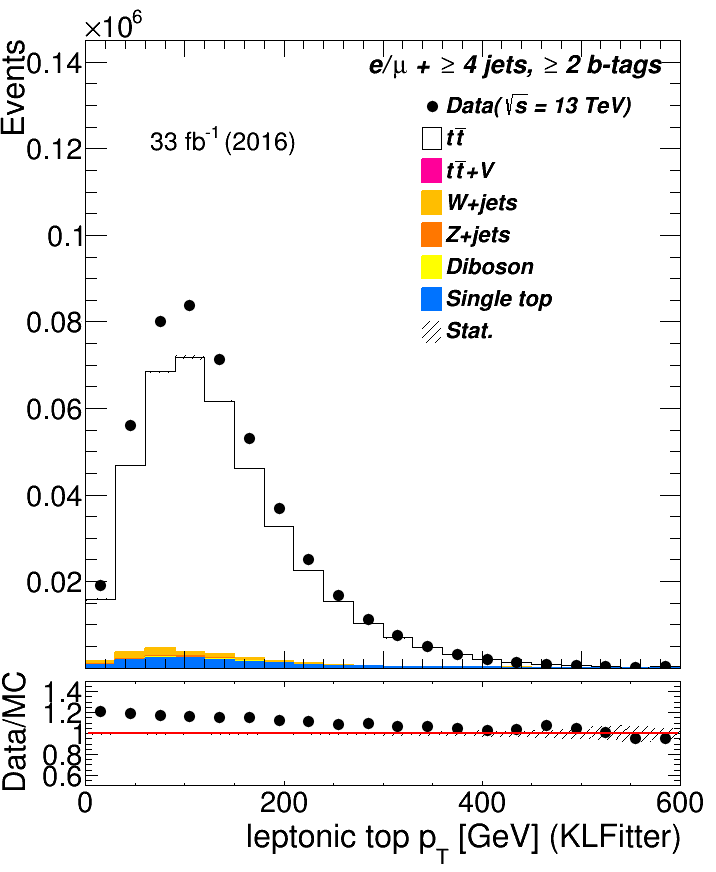
\includegraphics[width=\linewidth]{ControlPlots_emujets_2016_4incl_2incl/klf_topLep_pt_emujets_2016.png}
		\caption{Transverse momentum of the leptonic quark.} \label{fig:K15}
	\end{subfigure}	\hspace*{0.5cm}
	\begin{subfigure}{0.25\textwidth}
		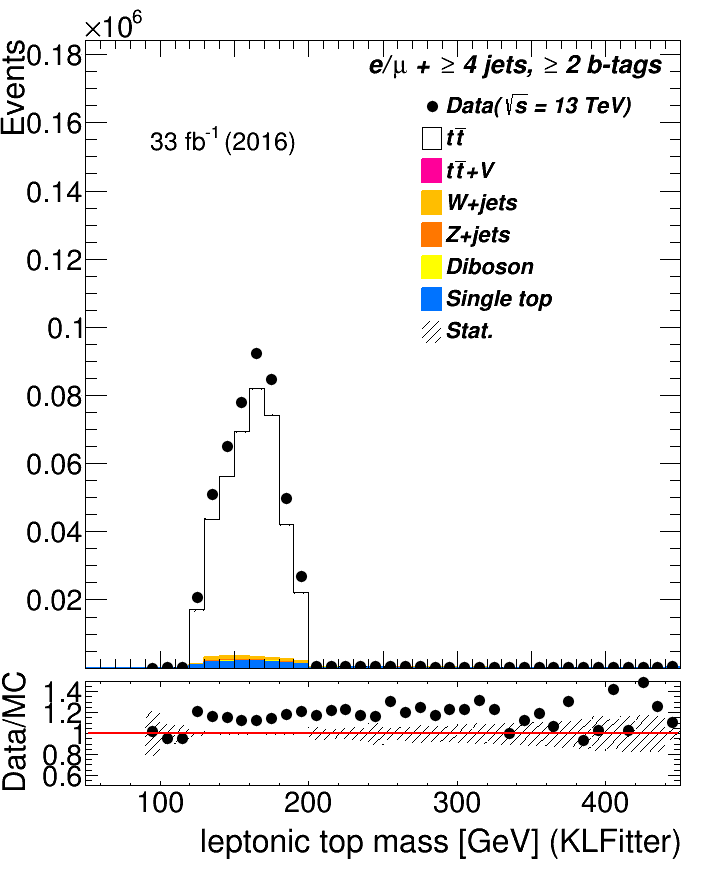
\includegraphics[width=\linewidth]{ControlPlots_emujets_2016_4incl_2incl/klf_topLep_m_emujets_2016.png}
		\caption{ Invariant mass of the leptonic top quark.} \label{fig:K16}
	\end{subfigure}\hspace*{0.25cm}
	\begin{subfigure}{0.25\textwidth}
		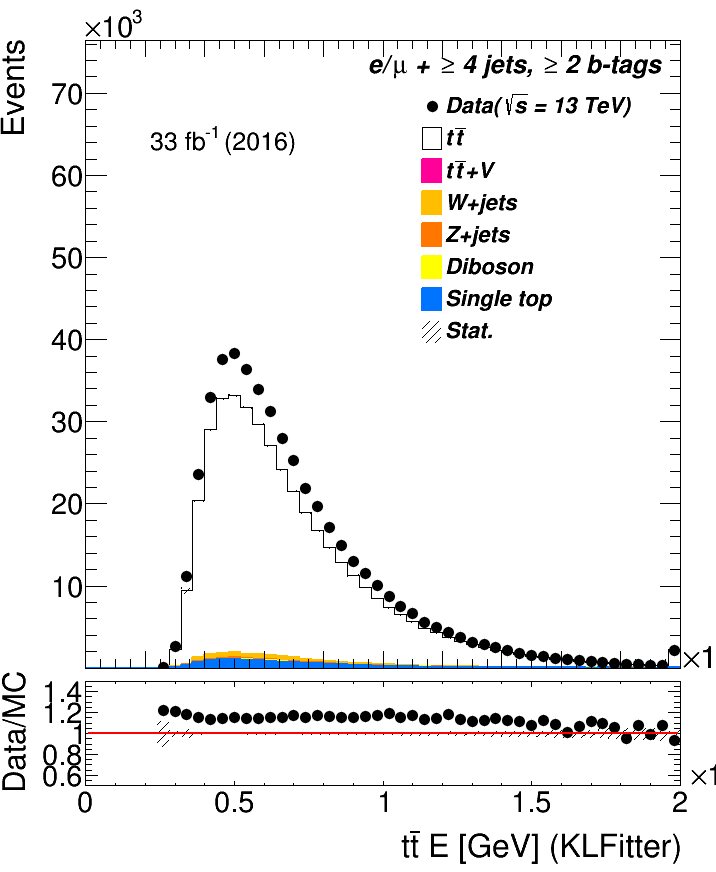
\includegraphics[width=\linewidth]{ControlPlots_emujets_2016_4incl_2incl/klf_ttbar_E_emujets_2016.png}
		\caption{Energy of the top-quark pair.} \label{fig:K17}
	\end{subfigure}


	\begin{subfigure}{0.25\textwidth}
		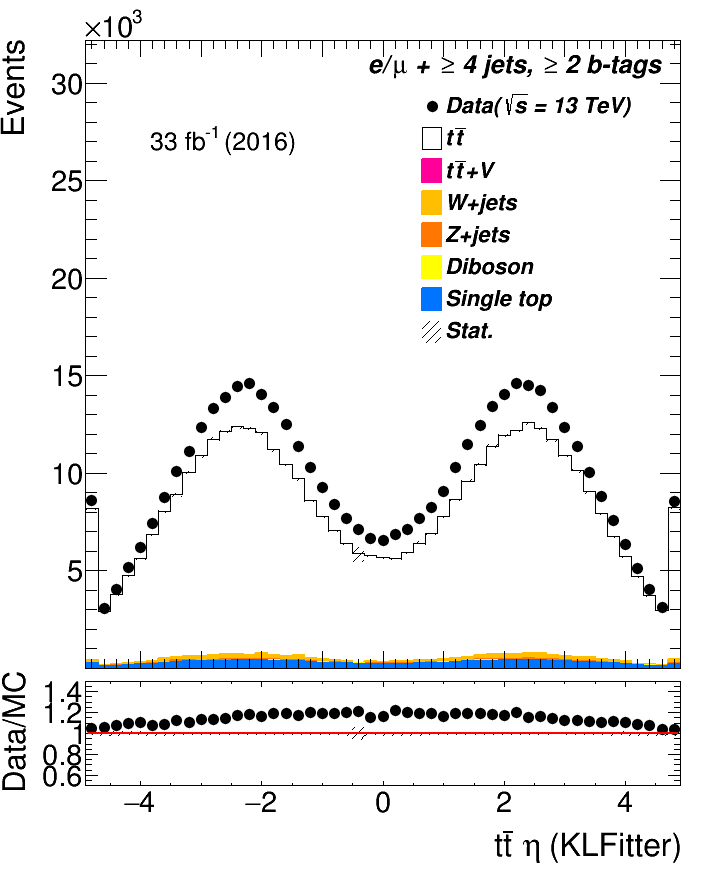
\includegraphics[width=\linewidth]{ControlPlots_emujets_2016_4incl_2incl/klf_ttbar_eta_emujets_2016.png}
		\caption{Rapidity of the top-quark pair.} \label{fig:K18}
	\end{subfigure}
	\hspace*{0.5cm}
	\begin{subfigure}{0.25\textwidth}
		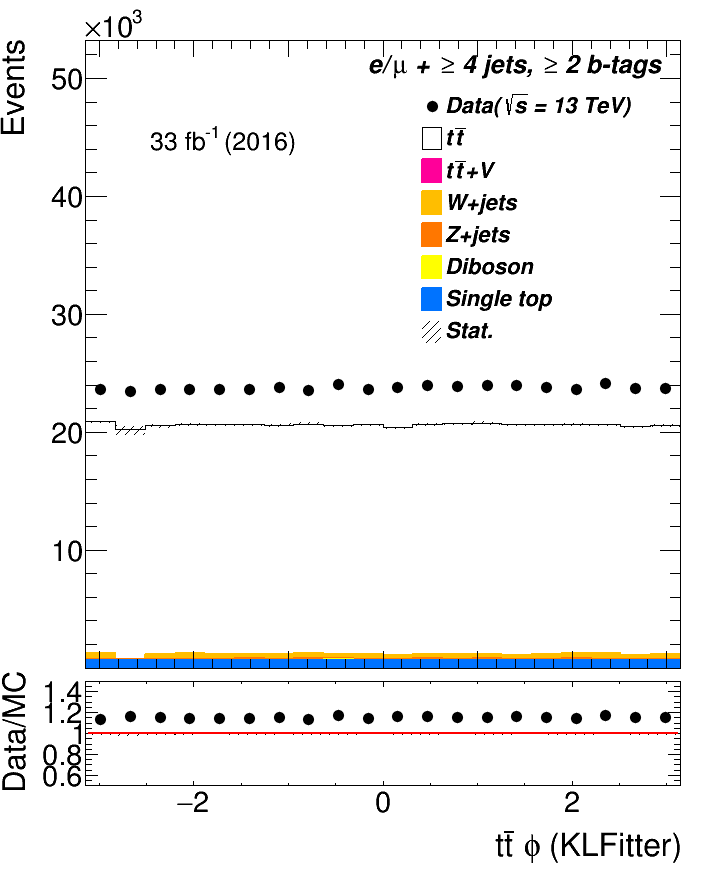
\includegraphics[width=\linewidth]{ControlPlots_emujets_2016_4incl_2incl/klf_ttbar_phi_emujets_2016.png}
		\caption{$\phi$  distribution of the top-quark pair.                       } \label{fig:K19}
	\end{subfigure}
\hspace*{0.5cm}
	\begin{subfigure}{0.25\textwidth}
		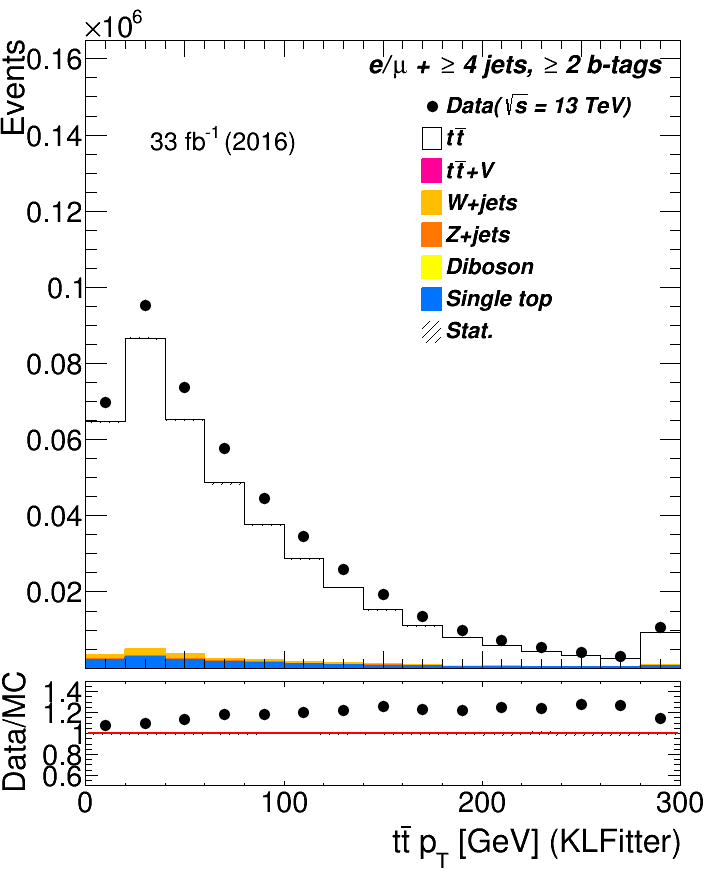
\includegraphics[width=\linewidth]{ControlPlots_emujets_2016_4incl_2incl/klf_ttbar_pt_emujets_2016.png}
		\caption{Transverse momentum of the top-quark pair.} \label{fig:K20}
	\end{subfigure}
	
	\caption{Same plots as for~\cref{klf100} of the  global properties of the leptonic and hadronic top-quark, as well as of the top-quark pair, reconstructed with \textsc{KLFitter}.  }
\end{figure}	




